\section{Optimization Targets}
\subsection{Power vs. Performance}
The two main targets to be considered when determining a scheduling policy are power and performance.
These also represent the primary tradeoff in scheduling on asymmetric multiprocessors.
There can be two extremes regarding these targets: 100\% performance and 0\% power efficiency, or 0\% performance and 100\% power efficiency.
If a scheduling policy is executing to achieve maximum power efficiency, tasks will execute sequentially on the most power-efficient core.
This policy will result in the longest runtime of all possible options.
If a scheduling policy is executing to achieve maximum performance, tasks will get allocated on the fastest core first with other tasks placed on the slower cores if possible.
This is the fastest na\"ive policy, and will use the most power and energy. \cite{AAP2013}

Ideally, the scheduling policy should lie somewhere in the middle between these two extremes, at least for mobile devices \cite{AAP2013}.
This tradeoff can is visualised in figure \ref{fig:PowerVSPerformance}.
Note that power is measured in bogowatts and time is measured in seconds.
\begin{figure}[h]
	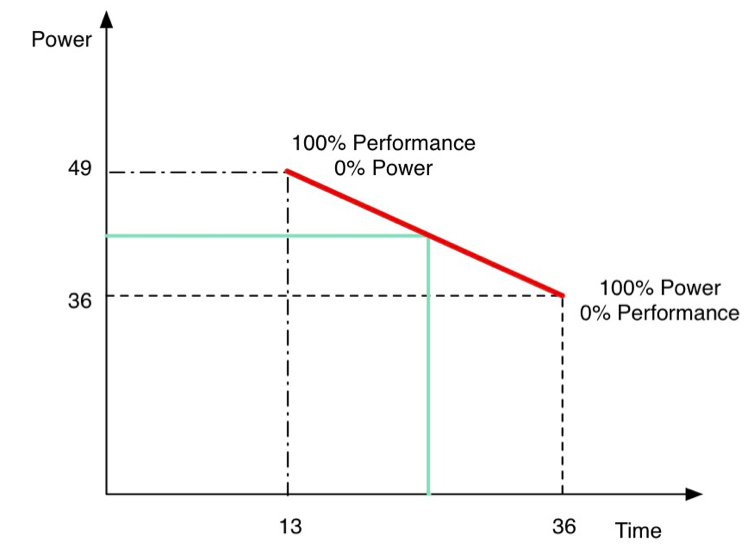
\includegraphics[width=\textwidth]{images/power_vs_performance.jpg}
	\caption{Power vs. Performance \cite{AAP2013}}
	\label{fig:PowerVSPerformance}
\end{figure}